\ffigbox[\FBwidth]{%
\caption{\centering Graphe représenté à partir de \(uv\)\\(les %
autre sommets peuvent être reliés à ceux\\ de l'autre %
côté mais pas entre eux)}\label{Fig:dm1ex3q2}
}{
    \fbox{
        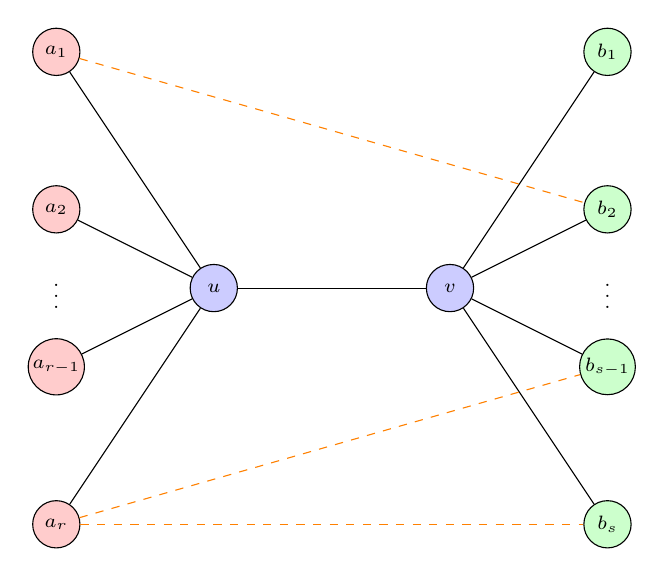
\begin{tikzpicture}[scale=1, every node/.style={circle, draw, fill=blue!20, inner sep=1pt, font=\scriptsize, minimum size=6mm}]
            % les deux sommets initiaux
            \node (u) at (0,0) {\(u\)};
            \node (v) at (3,0) {\(v\)};

            % ceux liés à u
            \node[fill=red!20] (a1) at (-2,3) {\(a_1\)};
            \node[fill=red!20] (a2) at (-2,1) {\(a_2\)};
            \node[fill=red!20] (a3) at (-2,-1) {\(a_{r-1}\)};
            \node[fill=red!20] (a4) at (-2,-3) {\(a_{r}\)};

            % ceux liés à v
            \node[fill=green!20] (b1) at (5,3) {\(b_1\)};
            \node[fill=green!20] (b2) at (5,1) {\(b_2\)};
            \node[fill=green!20] (b3) at (5,-1) {\(b_{s-1}\)};
            \node[fill=green!20] (b4) at (5,-3) {\(b_{s}\)};
            % on relie les sommets
            \foreach \x in {1,2,3,4} {
                \draw (u) -- (a\x);
                \draw (v) -- (b\x);
            }

            % on relie u et v
            \draw (u) -- (v);

            % on relie fictivement d'autres sommets
            \draw[orange, dashed] (a1) -- (b2);
            \draw[orange, dashed] (a4) -- (b3);
            \draw[orange, dashed] (a4) -- (b4);


            % on rajoute les ellipses
            \node[draw=none, fill=none] at (-2,0) {\(\vdots\)};
            \node[draw=none, fill=none] at (5,0) {\(\vdots\)};
        \end{tikzpicture}
    }
}